\documentclass[10pt]{article}
\usepackage{graphicx}
\usepackage{amssymb,amsmath}
\usepackage{siunitx}
\usepackage[a4paper]{geometry}
\usepackage{amsmath}
\usepackage{multirow}
\usepackage{hyperref}
\usepackage{color}
\usepackage{tabularx}
\usepackage{multirow}
\usepackage{supertabular}

% Bibliography
\usepackage[style=alphabetic,sorting=nyt,sortcites=true,autopunct=true,babel=hyphen,hyperref=true,abbreviate=false,backref=true,backend=biber]{biblatex}
\addbibresource{FLIPPERDOC.bib} % BibTeX bibliography file
\defbibheading{bibempty}{}

% Index
\usepackage{calc} % For simpler calculation - used for spacing the index letter headings correctly
\usepackage{makeidx} % Required to make an index
\makeindex % Tells LaTeX to create the files required for indexing


\begin{document}

\begin{titlepage}

\newcommand{\HRule}{\rule{\linewidth}{0.5mm}} % Defines a new command for the horizontal lines, change thickness here

\center % Center everything on the page
 
%----------------------------------------------------------------------------------------
%	HEADING SECTIONS
%----------------------------------------------------------------------------------------

\textsc{\LARGE Team FLIPPER presents}\\[1.5cm] % Name of your university/college
\vspace{3cm}
\textsc{\Large A short manual for}\\[0.5cm] % Major heading such as course name

%----------------------------------------------------------------------------------------
%	TITLE SECTION
%----------------------------------------------------------------------------------------

\HRule \\[0.4cm]
%{ \huge \bfseries FLIPPER}\\[0.4cm] % Title of your document

\includegraphics[width=\linewidth]{FLIPPERDOC_Figures/Logo_FLIPPER.png}\\[0.1cm]
\HRule \\[1.5cm]
 
%----------------------------------------------------------------------------------------
%	AUTHOR SECTION
%----------------------------------------------------------------------------------------

\begin{minipage}{0.4\textwidth}
\begin{flushleft} \large
\emph{Author:}\\
Sebastiaan \textsc{van de Velde} % Your name
\end{flushleft}
\end{minipage}
~
\begin{minipage}{0.4\textwidth}
\begin{flushright} \large
\emph{With input from:} \\
... \textsc{...} % Supervisor's Name
\end{flushright}
\end{minipage}\\[2cm]

% If you don't want a supervisor, uncomment the two lines below and remove the section above
%\Large \emph{Author:}\\
%John \textsc{Smith}\\[3cm] % Your name

%----------------------------------------------------------------------------------------
%	LOGO SECTION
%----------------------------------------------------------------------------------------

%
\includegraphics[width=\linewidth]{FLIPPERDOC_Figures/Logo_FLIPPER.png}\\[0.1cm] % Include a department/university logo - this will require the graphicx package

%----------------------------------------------------------------------------------------
%	DATE SECTION
%----------------------------------------------------------------------------------------
\vspace{2cm}
{\large \today}\\[3cm] % Date, change the \today to a set date if you want to be precise

 
%----------------------------------------------------------------------------------------

\vfill % Fill the rest of the page with whitespace

\end{titlepage}
\pagenumbering{roman}
\setcounter{tocdepth}{3}
\tableofcontents
\pagebreak
\setcounter{page}{1}
\pagenumbering{arabic}


\section{Introduction}
FLIPPER (short for: FLexible Interpretation of Porewater Profiles and Estimation of Rates) has been initially created to be able to analyze porewater data in sediments that are colonized by cable bacteria. Because of the electrical fields that are created by the long-distance electron transport, traditional programs (such as the original PROFILE program of \cite{Berg1998}) are not able to directly derive rates in electro-active sediments (i.e. sediments with an active electrical field). This is because they generally fit the steady state mass balance equation
\begin{equation}
 \frac{\delta}{\delta x} \left[\phi\left(D_s+D_B \right) \frac{\delta C}{\delta x}\right] + \phi \alpha \left( C_0-C\right) +R= 0
 \label{eq_diageq}
\end{equation}
where $\phi$ is the porosity, $x$ is the depth coordinate, $C$ is the pore-water concentration, $C_0$ is the bottom-water concentration, $\alpha$ is the bio-irrigation coefficient, $D_s$ is the effective diffusion coefficient of the solute (i.e. corrected for porosity) and $D_B$ is the bio-diffusion coefficient. 
The problem for electro-active sediments is that dissolved ions also undergo advection due to the electrical field \cite{RisgaardPetersen2012}. In these sediments, the flux of an ion is given by the Nernst-Planck equation \cite{RisgaardPetersen2012}
\begin{equation}
 J = -\phi D_S\frac{\delta C}{\delta x} + I
 \label{eq_nernstplanck}
\end{equation}
where $I$ is the ionic drift term and defined as
\begin{equation}
I=-\phi D_s z \frac{FE}{RT}C
 \label{eq_ionicdrift}
\end{equation}
where $F$ is the faraday constant, $R$ is the universal gas constant, $T$ is the absolute temperature and $z$ denotes the charge of the ion (negative for anions and positive for cations). The electrical field vector $E$ by convention points from a positively charged domain to a negatively charged domain. Since we introduce the electrical field strength as the length of the field vector ($E=||E||$), we include a negative sign in eq. \ref{eq_ionicdrift}, as for cable bacteria, the deeper sediment is positively charge (consumption of electrons by anodic sulfide oxidation). So the correct form of eq. \ref{eq_diageq} for electro-active sediments then becomes
\begin{equation}
 \frac{\delta}{\delta x} \left[\phi\left(D_s+D_B \right) \frac{\delta C}{\delta x} - I \right] + \phi \alpha \left( C_0-C\right) +R= 0
 \label{eq_diagelectroactiveeq}
\end{equation}
If you use the PROFILE program, it is necessary to afterwards correct for the ionic drift term, which is theoretically possible but not the most elegant solution (see the *extended* supplementary information sections of \cite{vandeVelde2016} and \cite{vandeVelde2017}). For that reason it was decided we would build our own program, which can deal with ionic drift in marine sediments.

Aside from being able to to discrete analysis of pore-water profiles, we included two other functions. The 'gradient' function allows you to quickly calculate diffusive fluxes, whereas the 'continuous' function is a novel method. This analysis method is based on the mathematics of spectral analysis, and more specifically Savitzky-Golay filtering \cite{Savitzky1964}. This latter procedure, while very promising and advanced, is not extensively tested - so it is advised to use it always together with the discrete analysis - especially when analysing coarser resolution profiles (i.e., sediment sliced at 0.5cm intervals). You will see that (most of the time) results are very similar. In what follows, we will give a short overview of what to provide as input, and what you will get as output. This will be far from complete, but questions/remarks can always be directed to us (\textbf{sebastiaan.van.de.velde@ulb.be}). In fact, any bugs you might spot would help greatly in increasing the perfomance of FLIPPER, while things that are unclear will help write this manual - so please do tell us what goes wrong!

\section{Required software and packages}
\label{sect_software}

FLIPPER is a series of functions and scripts to analyze porewater profiles of dissolved species. It is written in the R language, so you will need a functioning version of R and Rstudio. Since it is not made into an official package, you will need to download the folder directly from its github home (https://github.com/sevdevel/FLIPPER.git). This can be done either via using a gitclient, or just downloading the files from a browser. It has not been extensively tested on different platforms (only on windows and linux).

FLIPPER uses a series of R-packages that are essential for its functioning, so you need makes sure the following packages have installed on R:
\begin{itemize}
%\item tcltk (basepackage)
\item marelac
\item signal
\item fractaldim
\item ReacTran
\item marelac
\item FME
\item wavelets
\end{itemize}
Once those are installed, you just need to 'source' the two main functions. Make sure your working directory is the FLIPPER directory, because sourcing the two main functions will lead to sourcing all the others, and their paths are given relative to the main functions (something we will have to change in the future);
\begin{verbatim}
source("FLIPPER_plotfunction.R")
source("user interface function.R")
\end{verbatim}
Then change back to your working directory and start analyzing ...

\section{FLIPPER}
\label{sect_functioning}
FLIPPER is called as follows:
\begin{verbatim}
FLIPPER.func(input,por.cte=NA,E.cte=NULL,tort.dep=1,species,method=NULL,
             env.parms=NULL,full.output=FALSE,
             discrete.parms=NULL,
             continuous.parms=NULL,
             gradient.parms=NULL)
\end{verbatim}

\subsection{"input": data input dataframe}
At the bare minimum, you need to supply it with an input dataframe containing depth and concentrations and a porosity value (either as a constant value, or included in the input dataframe). All other arguments have default values that allow FLIPPER to run. The file "userInterface example.R" provides an example on how to run FLIPPER. It loads some dummy datasets, and analyzes those with FLIPPER. You can start there to explore how the input is provided.

The most important input is the "input" dataframe. This contains at least 2 columns: \textit{x} and \textit{C} (not the capitalization of C), which stands for depth (\textit{x}, in $m$) and concentration (\textit{C}, in $mmol \: m^{-3}$). A basic input dataframe would look like
\begin{verbatim}
     x    C
0.0000   39
0.0025  260
0.0075  648
0.0125 1118
0.0175 1178
0.0225 2120
\end{verbatim}  



You can also add a porosity column (\textit{por}, unitless) to the input dataframe, so it would look something like
\begin{verbatim}
     x    C  por
0.0000   39 1.00
0.0025  260 0.81
0.0075  648 0.74
0.0125 1118 0.74
0.0175 1178 0.74
0.0225 2120 0.73
\end{verbatim}
It is important to remember that if you do not supply porosity in the input dataframe, it needs to be supplied as a constant (\textit{por.cte}) in the FLIPPER function call. 

Other columns that can be included are electrical field (\textit{E}), advective velocity (\textit{v}), first derivative of porosity (\textit{dpor\_dx}), first derivative of advective velocity (\textit{dv\_dx}) and first derivative of the effective diffusion coefficient (\textit{dDs\_dx}). The latter three columns are only relevant for the continuous analysis.

\begin{table*}[!h]
	\small
	\caption{Possible columns in the input dataframe for FLIPPER}
	\begin{tabular}{p{5cm} p{1.5cm} p{2cm} p{2cm}}
		\hline
		\textbf{Parameter} & \textbf{Symbol} & \textbf{Unit} & \textbf{Default} \\     
		 \hline
		\textbf{Depth} & x & $m$ & -  \\
		\textbf{Concentration} & C & $mmol \: m^{-3}$ & -  \\
		\textbf{Porosity} & por & - & -  \\
		\textbf{Electrical field} & E & $V \: m^{-1}$ & -  \\
		\textbf{Advective velocity} & v & $m \: d^{-1}$ & -  \\
		\textbf{First derivative of porosity} & dpor\_dx & $m^{-1}$ & -  \\
		\textbf{First derivative of advective velocity} & dv\_dx & $d^{-1}$ & -  \\
		\textbf{First derivative of the effective diffusive coefficient} & dDs\_dx & $m \: d^{-1}$ & -  \\
		\hline
	\end{tabular}
	\label{table_inputdf}
\end{table*}


\subsection{single value input parameters}
The \textit{species} input value is required, so FLIPPER knows which species it is analyzing (so it can calculate the diffusion coefficient - which it does using the CRAN:marelac package \cite{Soetaert2010}). This is supplied as a character vector, e.g.,
\begin{verbatim}
c("O2")
c("Fe2+")
\end{verbatim}

If you have chosen not to include porosity in the input dataframe, you have to supply a constant porosity value \textit{por.cte}. 

You can also supply an electrical field as a vector instead of a continuous profile. This is done via the \textit{E.cte} parameter, which you should apply with a vector of length three; the strength of the electrical field (in $V \: m^{-1}$), the start depth of the electrical field and the end depth of the electrical field. An input vector for \textit{E.cte} would then look like
\begin{verbatim}
c("value.E","start.depth","end.depth)
c(-0.1,0.0,0.03)
\end{verbatim}

You are given the option to choose which tortuosity correction you want, by supplying an integer value between 1 and 4 in \textit{tort.dep}. The options are
\begin{equation}
tort.dep=1: 1-2ln(por) \:: (default) 
\end{equation}
\begin{equation}
tort.dep=2: por^{-1} 
\end{equation}
\begin{equation}
tort.dep=3: por^{-2} 
\end{equation}
\begin{equation}
tort.dep=4: 1+3(1-por)
\end{equation}

And finally, you can choose which method you want to apply via \textit{method}. Options are "all" (or NULL) - which will run all three methods - "gradient", "discrete" or "continuous" - which, we hope, speak for themselves.

\subsection{"env.parms": environmental parameters list}
All environmental parameters are optional. However, we would advise to supply as much as possible - in particular with respect to the environmental parameters. These are provided as a list called "env.parms", which contains temperature (\textit{TC}, in $\deg C$), salinity (\textit{S}, unitless), pressure (\textit{P}, in bar), diffusive coefficient (\textit{Dmol}, in $m^2 \: d^{-1}$) and charge of the ion (\textit{z}). An env.parms list that contains temperature and salinity would then look like (if you printed it in R)
\begin{verbatim}
$TC
[1] 10

$S
[1] 30
\end{verbatim} 
The diffusive coefficient is calculate from temperature, salinity and pressure using the CRAN:marelac package \cite{Soetaert2010}. However, if you are analyzing a compound whose diffusion coefficient is not included in marelac, you can supply the diffusion coefficient manually.

\begin{table*}[!h]
	\small
	\caption{Environmental parameters in the env.parms list for FLIPPER}
	\begin{tabular}{p{5cm} p{1.5cm} p{2cm} p{2cm}}
		\hline
		\textbf{Parameter} & \textbf{Symbol} & \textbf{Unit} & \textbf{Default} \\     
		 \hline
		\textbf{Temperature} & TC & $\deg C$ & 10.0  \\
		\textbf{Salinity} & S & - & 30.0  \\
		\textbf{Pressure} & P & $bar$ & 1.013  \\
		\textbf{Diffusive coefficient} & Dmol & $m^2 \: d^{-1}$ & -  \\
		\textbf{Charge of the ion} & z & - & 0  \\
		\hline
	\end{tabular}
	\label{table_envparms}
\end{table*}

\subsection{"gradient.parms": gradient parameters list}
The only parmater that can be supplied to the gradient parameter list is \textit{x.limits}, which determines between which points the gradient has to be calculated. If this is not supplied, an interactive window will be plotted which lets you select the points you want interactively.

\begin{table*}[!h]
	\small
	\caption{Gradient parameters in the gradient.parms list for FLIPPER}
	\begin{tabular}{p{8cm} p{1.5cm} p{1cm} p{1cm}}
		\hline
		\textbf{Parameter} & \textbf{Symbol} & \textbf{Unit} & \textbf{Default} \\     
		 \hline
		\textbf{Limits between which gradient is calculated} & x.limits & $m$ & -  \\
		\hline
	\end{tabular}
	\label{table_gradientparms}
\end{table*}

\subsection{"discrete.parms": discrete parameters list}
The discrete parameter list gives you the opportunity to control how the analysis is done. The most important parameters here are \textit{x.up} and \textit{L.down}, which decide the upper (\textit{x.up}) and the lower (\textit{L.down}) bound of the profile that has to be analyzed. By default it takes the topmost value in the sediment, and the lowest value. You can also decide which boundary conditions you want, which is controlled by the parameterser \textit{UBC} and \textit{LBC}. Possible values are "flux.up" and "conc.up" for \textit{UBC} and "no.flux", "conc.down" and "flux.down" for \textit{LBC}. "conc.up" and "conc.down" boundary conditions take the uppermost and lowermost concentration as values. If you choose a fixed flux, you have to provide the respective fluxes in \textit{flux.up} and \textit{flux.down} parameter set.

Other possible parameters are \textit{i.end} and \textit{initial.zones}, which determine the maximum numbers of zones that will be test (\textit{i.end}), or from what number of zones the lumping should start (\textit{initial.zones}).

\begin{table*}[!h]
	\small
	\caption{Discrete parameters in the discrete.parms list for FLIPPER. $^{1}$only for positive values (ignores values in the watercolumn). $^{2}$Or the number of discrete measurements - 2, whichever is smallest. $^{3}$Only taken into account when "flux.up" or "flux.down" is selected as boundary condition.}
	\begin{tabular}{p{8cm} p{1.5cm} p{2cm} p{2cm}}
		\hline
		\textbf{Parameter} & \textbf{Symbol} & \textbf{Unit} & \textbf{Default} \\     
		 \hline
		\textbf{Lower boundary of the integration domain } & L.down & $m$ & max(input\$x)$^{1}$  \\
        \textbf{Upper boundary of the integration domain} & x.up & $m$ & min(input\$x)$^{1}$  \\	
        \textbf{Number of layers for the fitting function} & N & - & 200  \\	
        \textbf{Maximum number of discrete production zones to test} & i.end & - & 12$^{2}$  \\	
        \textbf{Number of zones to start lumping } & initial.zones & - & -  \\	
        \textbf{Probability with which the null hypothesis is rejected} & p & - & 0.01  \\	
        \textbf{Upper boundary condition} & UBC & - & "conc.up"  \\	
        \textbf{Lower boundary condition} & LBC & - & "no.flux"  \\	
        \textbf{Flux across the upper boundary} & flux.up & $mmol \: m^{-2} \: d^{-1}$ & -$^{3}$   \\
        \textbf{Flux across the lower boundary} & flux.down & $mmol \: m^{-2} \: d^{-1}$ & -$^{3}$  \\
		\hline
	\end{tabular}
	\label{table_discreteparms}
\end{table*}

\subsection{"continuous.parms": continuous parameters list}
For the continuous function, we currently recommend to not change anything away from their default value.


\begin{table*}[!h]
	\small
	\caption{Continuous parameters in the continuous.parms list for FLIPPER.\\ $^{1}$ value is either  1, 2 or 3. Value = 1: no constraint on flux (default value). Value = 2: constant flux imposed. Value = 3: zero flux imposed. \\ $^{2}$ either "automated" or "interactive" (default). Interactive allows user to select ideal filter size, automated lets function select ideal filter size. The first is recommended for coarser profiles. \\ $^{3}$Either "average" or "interpolate" (default). Average (take maximum stepsize) or interpolate (take minimum stepsize)}
	\begin{tabular}{p{8cm} p{1.7cm} p{1cm} p{2.5cm}}
		\hline
		\textbf{Parameter} & \textbf{Symbol} & \textbf{Unit} & \textbf{Default} \\     
		 \hline
		\textbf{Order of the polynomial that is fitted} & p & - & 3  \\
        \textbf{Integer determining filter behaviour at the upstream (upper, left) boundary} & bnd.upper & - & 1$^{1}$  \\	
        \textbf{Integer determining filter behaviour at the downstream (lower, right) boundary} & bnd.lower & - & 1$^{1}$  \\	
        \textbf{Window size used in filtering the concentration C / flux J / production R, representing the number of data points to the left and right of the data midpoint} & n.C, n.J, n.R & - & NULL  \\	
        \textbf{Determination of optimal window size} & optimal.window.size & - & "interactive"$^{2}$   \\	
        \textbf{Take a uniform filtering window for C, J and R} & n.uniform & - & FALSE  \\
        \textbf{Minimum value of the window size, used when scanning the optimal window size} & min.n & - & p - p\%\%2  \\	
        \textbf{Maximum value of the window size, used when scanning the optimal window size} & max.n & - & nrow(input)\%/\%2 - 1  \\	
        \textbf{Keeps windows created by automated function} & keep.graphics & - & FALSE  \\	
        \textbf{Create equidistant data points} & interpolation & - & "interpolate"$^{3}$  \\

		\hline
	\end{tabular}
	\label{table_continuousparms}
\end{table*}

\section{Output}
Once run succesfully, FLIPPER will provide a list as output. This list will contain (if applicable):
\begin{itemize}
\item \textit{method}: the method chosen
\item \textit{input}: a list which contains
\begin{itemize}
 \item \textit{user.input}: a list with user.input: the user supplied dataframe (x, C, por, tort ...)
 \item \textit{continuous.input}: the interpolated dataframe for use in the continuous function
\end{itemize}
\item \textit{parms}: a list which contains
\begin{itemize}
 \item \textit{env.parms}: list with the inputted environmental parameters (default with user supplied)
 \item \textit{gradient.parms}: the output of the gradient function
 \item \textit{discrete.parms}:  the parameters supplied in the discrete function
 \item \textit{continuous.parms}: the parameters used in the continuous function
\end{itemize}
\item \textit{output}: a list which contains
\begin{itemize}
 \item \textit{gradient.output}: the output of the gradient function
\begin{itemize}
\item  \textit{J.dif.up}: the diffusive flux
\item  \textit{J.adv.up}: the advective flux
\item  \textit{R.int}: the integrated reaction rate
\item  \textit{fit}: details about the linear fit (from the R function 'lm')
\end{itemize}
  \item \textit{discrete}:  the output of the discrete function
\begin{itemize}
\item  \textit{J.dif.up}: the diffusive flux at the top of the domain
\item  \textit{J.adv.up}: the advective flux at the top of the domain
\item  \textit{J.dif.down}: the diffusive flux at the bottom of the domain
\item  \textit{J.adv.down}: the advective flux at the bottom of the domain
\item  \textit{R.vol}: the volumetric reaction rate
\item  \textit{R.int}: the integrated reaction rate
\item  \textit{fit}: the selected model fit 
\end{itemize}
 \item \textit{continuous}: the output of the continuous function
 \begin{itemize}
\item  \textit{J.dif.up}: the diffusive flux at the top of the domain
\item  \textit{J.adv.up}: the advective flux at the top of the domain
\item  \textit{J.dif.down}: the diffusive flux at the bottom of the domain
\item  \textit{J.adv.down}: the advective flux at the bottom of the domain
\item  \textit{R.int}: the integrated reaction rate
\item  \textit{overview}: the derived concentration, flux and reaction profiles
\end{itemize}
\end{itemize}

\end{itemize}

\section{Visualisation}

FLIPPER also contains an easy plot.function, which is called as
\begin{verbatim}
plot.FLIPPER(output)
\end{verbatim}
where you provide the output structure generated by FLIPPER.func. An example of such a plot is given in Fig. \ref{fig_Flipperplot}.

\begin{figure}[!htbp]
	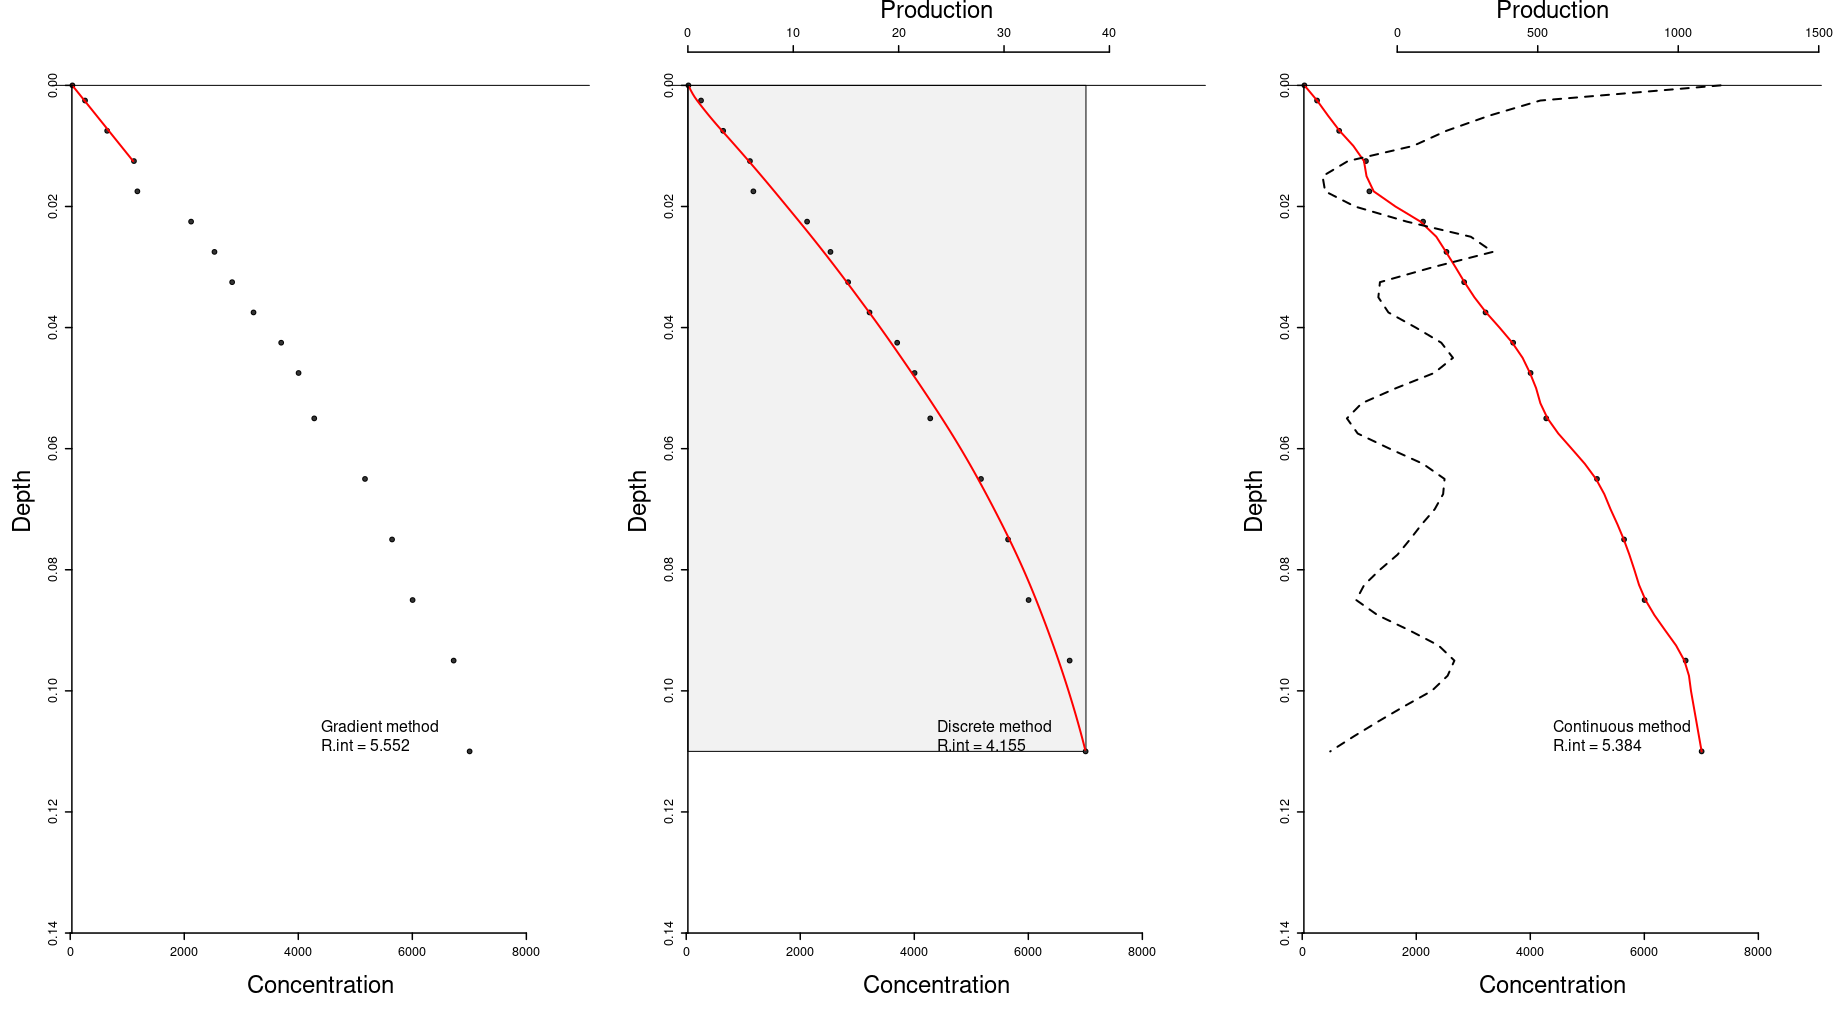
\includegraphics[width=\linewidth]{FLIPPERDOC_Figures/FLIPPER_plotexample.png}
	\caption{Example of a FLIPPER plot.}
	\label{fig_Flipperplot}
\end{figure}



\section{References}
\begin{thebibliography}{}
	
\bibitem[Bergetal.(1998)]{Berg1998}
Berg, P., Risgaard-Petersen, N., and Rysgaard, S.:Interpretation of measured concentration profiles in sediment pore water, Limnology and Oceanography, 1998, 1500-1510. doi:10.4319/lo.1998.43.7.1500
	
\bibitem[RisgaardPetersenal.(2012)]{RisgaardPetersen2012}
Risgaard-Petersen, N., Revil, A., Meister, P., and Nielsen, L.P.: Sulfur, iron, and calcium cycling associated with natural electric currents running through marine sediment, Geochimica et Cosmochimica Acta, 2012, 92:1-13. doi:10.1016/j.gca.2012.05.036

\bibitem[SavitskyandGolay(1964)]{Savitzky1964}
Savitzky, A., and Golay, M.J.E.: Smoothing and Differentiation of Data by Simplified Least Squares Procedures, Analytical Chemistry, 1964, 36:1627-1639. doi:10.1021/ac60214a047

\bibitem[Soetaertetal.(2010)]{Soetaert2010}
Soetaert, K., Petzoldt, T., and Meysman, F.J.R.: marelac: Tools for Aquatic Sciences R package version 2.1

\bibitem[vandeVeldeal.(2016)]{vandeVelde2016}
van de Velde, S., Lesven, L., Burdorf, L.W., Hidalgo-Martinez, S., Geelhoed, J.S., Van Rijswijk, P., Gao, Y., and Meysman F.J.R.: The impact of elecrogenic sulfur oxidation on the biogeochemistry of coastal sediments: A field study, Geochimica et Cosmochimica Acta, 2016, 194:211-232. doi:10.1016/j.gca.2016.08.038

\bibitem[vandeVeldeal.(2017)]{vandeVelde2017}
van de Velde, S., Callebaut, I., Gao, Y., and Meysman F.J.R.: Impact of elecrogenic sulfur oxidation on trace metal cycling in a coastal sediment, Chemical Geology, 2017, 452:9-23. doi:10.1016/j.chemgeo.2017.01.028
		
\end{thebibliography}

\section{FAQ and useful svn/linux commands}

\end{document}
